\begin{boxK}
    \lr{
        \lstinputlisting[language = Python]{Final/code/encrypt1.py}
    }
\end{boxK}


\begin{boxB}
    اولین کد، یک تابع برای رمزنگاری داده استفاده می‌شود. این الگوریتم بر روی بلوک‌های ثابتی از داده‌های ورودی عمل می‌کند. داده‌ی ورودی به دو نیمه ۳۲ بیتی تقسیم شده و سپس ۱۶ بار رمزنگاری انجام می‌شود. در هر بار از ۱۶ بار، مقدار "L" با یک مقدار از آرایه "p" XOR می‌شود، سپس به تابع "calculate" ارسال شده و نتیجه‌ی این تابع با "R" XOR می‌شود. سپس مقادیر "L" و "R" جابه‌جا می‌شوند. پس از انجام ۱۶ بار این عملیات، مقادیر "L" و "R" نهایی با دو مقدار از آرایه "p" XOR می‌شوند، سپس به یکدیگر متصل شده و به عنوان خروجی رمزنگاری شده برگردانده می‌شوند.
\end{boxB}


\begin{boxK}
\lr{
\lstinputlisting[language = Python]{Final/code/calculate1.py}
}
\end{boxK}


\begin{boxB}
    در کد دوم، تابع "calculate" پیاده‌سازی شده است. این تابع یک عملیات جایگزینی ساده است که یک عدد ۳۲ بیتی را به عنوان ورودی دریافت می‌کند و یک عدد ۳۲ بیتی را به عنوان خروجی بازگردانده می‌کند. این تابع از چهار جدول جستجو با طول ۲۵۶ ورودی خود را جایگزینی می‌کند. برای اینکار، ورودی به چهار بخش ۸ بیتی تقسیم شده و هر بخش به عنوان اندیس یکی از جداول جستجو انتخاب می‌شود. سپس مقدار ۳۲ بیتی متناظر با هر بخش از جدول برگردانده می‌شود. این چهار مقدار پس از اعمال عملیات XOR و جمع، به عنوان خروجی تابع بازگردانده می‌شوند. این نوع عملیات جایگزینی یک الگوریتم پرکاربرد در بسیاری از رمزنگاری‌های بلوکی است که با ترکیب چندین مرحله از جایگزینی و جابه‌جایی به داده‌های ورودی، سطح امنیت بالایی را فراهم
    می‌کند.
\end{boxB}

\begin{boxK}
    \lr{
        \lstinputlisting[language = Python]{Final/code/decrypt1.py}
    }
\end{boxK}

\begin{boxB}
    داده های عدد صحیح 64 بیتی را می گیرد و یک سری عملیات را برای رمزگشایی آن انجام می دهد.

ابتدا عدد صحیح 64 بیتی را به دو نیمه 32 بیتی L و R تقسیم می کند. سپس 16 بار در یک حلقه تکرار می شود و هر بار عملیات زیر را انجام می دهد:

XOR L با مقدار p[i] نتیجه را از طریق یک تابع محاسبه عبور دهید،
% که در قطعه کد تعریف نشده است و احتمالاً در جای دیگری تعریف شده است
XOR R با نتیجه تابع محاسبه اعمال شده به نتیجه عملیات XOR قبلی پس از تکمیل حلقه،
  مقادیر L و R، XORs L را با مقدار p[0] تعویض می کند،
XORs R با مقدار p[1]، و سپس آنها را به یک عدد صحیح 64 بیتی ترکیب می کند. عدد صحیح حاصل، نسخه رمزگشایی شده داده های ورودی است.

\end{boxB}

\begin{figure}[h]
    \centering
    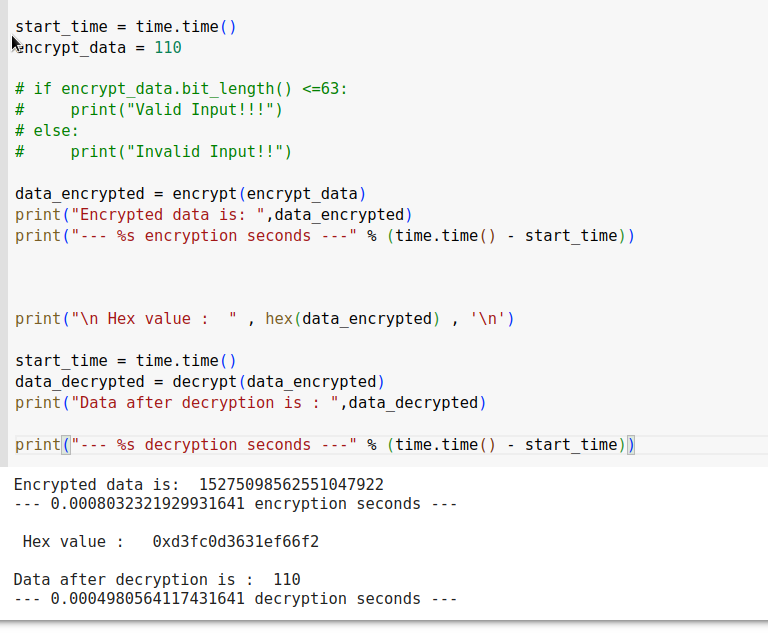
\includegraphics
    [width = 0.8\textwidth]
    {Final/images/blowfish.png}
    \caption{blowFish Algorithm}
    \label{fig:enter-label}
\end{figure}